% First manuscript draft. Main source for subsequent editing.
% Based on the supplied AAMAS 2027 template; class and layout unmodified.
\documentclass[sigconf,anonymous]{aamas}
\usepackage{balance}
\usepackage{tikz}
\usetikzlibrary{arrows.meta,positioning}
\makeatletter
\gdef\@copyrightpermission{
  \begin{minipage}{0.2\columnwidth}
   \href{https://creativecommons.org/licenses/by/4.0/}{
\includegraphics[width=0.90\textwidth]{by}}
  \end{minipage}\hfill
  \begin{minipage}{0.8\columnwidth}
   \href{https://creativecommons.org/licenses/by/4.0/}{This work is licensed under a Creative Commons Attribution International 4.0 License.}
  \end{minipage}
  \vspace{5pt}
}
\makeatother
\setcopyright{ifaamas}
\acmConference[AAMAS 2027]{Proc.\@ of the 26th International Conference
on Autonomous Agents and Multiagent Systems (AAMAS 2027)}{3--7 May 2027}{Hanoi, Vietnam}{M.~Baldoni, F.~Fang, W.~Yeoh, N.~Yorke-Smith (eds.)}
\copyrightyear{2027}
\acmYear{2027}
\acmDOI{}
\acmISBN{}
\acmSubmissionID{DRAFT}
\submissionType{Research Paper Track}
\title{When to Help: Scheduled and Physiology-Informed Assistance in Physical Tangram Solving}
\keywords{Human--robot interaction, adaptive assistance, intervention timing, physiological sensing, Wizard-of-Oz, tangram}
% Outstanding factual checks are kept in author-notes.md.
\citestyle{acmnumeric}

\begin{abstract}
In human--robot interaction (HRI), deciding when to provide assistance requires understanding how different intervention strategies affect both task performance and the user experience. Previous work has compared physiology-triggered robotic assistance with periodic support in surgical training. We extend this work to physical spatial problem solving by conducting a within-participant experiment to compare three conditions: no assistance, scheduled assistance, and adaptive assistance based on physiological signals. Twenty-four participants (N = 24) solve nine physical tangram puzzles across three sessions. The order of the conditions is varied across participants, and puzzles are randomly assigned to the sessions. Tangrams combine spatial reasoning with physical manipulation, providing a simple task for studying informational and physical assistance. Participants receive on-screen hints and robotic-arm interventions through a Wizard-of-Oz setup, with assistance either scheduled or adapted using heart-rate signals and task progress. We evaluate puzzle completion, completion time, workload, helpfulness, intervention timing, frustration, and trust. Both assistance conditions improve completion rates compared with no assistance; scheduled assistance achieves the highest completion and shortest duration, while adaptive assistance receives higher helpfulness and timing ratings and lower frustration. Together, these findings highlight distinct trade-offs between assistance strategies in task performance and user experience, providing insights for designing HRI systems that adapt assistance to the needs of the user.
\end{abstract}

\begin{document}
\maketitle

\section{Introduction}


A person solving a physical puzzle may stop moving for several reasons. They may be mentally rotating a piece, reconsidering an unsuccessful arrangement, or waiting because they do not know what to try next. These moments can look similar to an observer, yet call for different responses. A useful hint may let the person resume work; the same hint, delivered during a productive pause, may interrupt a solution they were about to reach. For an assistive robot, deciding when to act is therefore part of deciding how to help.

Human--robot interaction has long examined how people and robots coordinate their contributions to a shared task \cite{goodrich2007}. Recent work treats initiative as a decision that depends on the person's needs and the state of the task. For example, Andriella et al. model what assistance to offer, when to offer it, and how confidently to intervene \cite{andriella2025}. PACE uses estimates of human action completion to coordinate proactive robot assistance \cite{delazzari2025}. These approaches make timing an explicit part of collaboration. They also motivate a practical evaluation question: does an assistance strategy that supports efficient task execution also provide help that people consider appropriate?

Physiological signals offer an additional source of information for this decision. Yang et al. compared workload-based adaptive suction with periodic suction in a simulated surgical task \cite{yang2024}. Their study provides a direct precedent for comparing physiology-informed and time-based assistance. This comparison leaves open how a person will respond when assistance intervenes in a physical spatial problem, where help can affect both reasoning and manipulation. Moving a task object can change what is available for the person's next action, while a hint can change their understanding of the solution.

We examine this question using physical tangram puzzles. Participants must arrange seven geometric pieces to reproduce a target shape. The task combines spatial reasoning with manual manipulation and permits both written guidance and piece-level robotic assistance. It also provides an observable outcome: whether the target has been completed. Tangrams have previously been used as an HRI test scenario \cite{hirth2012}; our interest is in comparing assistance strategies within this setting rather than introducing tangrams as a new robotics task.

Three distinctions motivate the study. First, an unassisted condition is needed to separate the effect of receiving support from differences between two ways of providing it. Second, a completed puzzle does not reveal whether help felt useful or arrived at an appropriate moment, so performance and participant experience must be considered together. Third, a physiological cue and a decision to intervene are different events. Heart-rate changes alone do not establish that a participant needs assistance. In our system, the researcher interprets those cues alongside the participant's progress and retains control over the intervention.

We compare no assistance, scheduled assistance, and physiology-informed adaptive assistance in a within-participant design with nine puzzles arranged into three sittings. The same participant encounters all three conditions, with three different puzzles per condition. A Wizard-of-Oz interface coordinates the participant display, researcher dashboard, and robot-operator display. This arrangement allows us to study the interaction produced by the assistance strategies while keeping the human role in deciding and delivering assistance explicit.

The study addresses two questions. \textbf{RQ1:} How do the three assistance conditions differ in puzzle completion and task duration? \textbf{RQ2:} How do they differ in perceived workload and frustration, and how do the two assisted conditions compare in perceived helpfulness and intervention timing? These questions concern performance during the task; the study does not include a separate retention or transfer test from which to infer learning.

The work makes three contributions:

\begin{enumerate}
\item A comparison of unassisted, scheduled, and physiology-informed assistance within a shared physical spatial problem-solving task.
\item A Wizard-of-Oz platform that coordinates written hints, fixed robotic actions, physiological decision support, and a common record of task events.
\item An evaluation that pairs puzzle outcomes and duration with repeated assessments of workload and intervention experience, distinguishing per-puzzle responses from overall impressions of the system.

\end{enumerate}
\section{Related Work}

\subsection{Proactive assistance and coordination}

Assistive interaction requires a robot to coordinate its actions with a person's activity. Parasuraman et al. distinguish automation of information acquisition, analysis, decision selection, and action implementation \cite{parasuraman2000}. These functions can be automated to different degrees. In our setup, sensing and preliminary processing are automated, but intervention selection remains with the researcher. Newman et al. further distinguish reactive, proactive, and simultaneous assistance, making the timing of help an explicit design dimension \cite{newman2022}. The HRI literature places this coordination within broader questions of autonomy, communication, and the division of work \cite{goodrich2007}. An intervention policy determines more than whether assistance is available: it also determines the circumstances in which the robot takes the initiative.

Andriella et al. use influence diagrams to learn proactive assistance in a sequential memory game, explicitly representing the choice of assistance, intervention timing, and confidence \cite{andriella2025}. PACE approaches coordination through estimates of task progression derived from human hand movements and a learned assistance policy \cite{delazzari2025}. Both works connect robot action to the unfolding human activity. Our study examines a complementary design choice: how fixed scheduling and researcher-mediated use of physiological cues compare when the available assistance includes written hints and movement of physical puzzle pieces. The comparison evaluates the complete assistance strategies as enacted; it does not by itself isolate timing from differences in intervention frequency or content.

\subsection{Physiology-informed adaptation}

Workload-based assistance has been investigated in surgical human--robot collaboration. Yang et al. developed an adaptive suction tool and evaluated it against periodic suction in a simulated needle-passing task \cite{yang2024}. Their periodic interval was selected to approximate the assistance frequency observed in an earlier experiment. This is a relevant methodological distinction: comparing assistance timing requires attention to how much assistance each policy provides.

Related evidence comes from closed-loop human--robot teaming. Teo et al. found that assistance informed by individualized physiological workload models improved performance more than imposed aid \cite{teo2018}. In simulated driving, Luo et al. evaluated workload-adaptive haptic shared control using a workload estimate derived from gaze \cite{luo2021}. These studies motivate state-responsive assistance, but use sensing and control arrangements that differ from a wrist-sensor cue interpreted by a human researcher.

Physiological adaptation also requires care in the interpretation of its inputs. Delliaux et al. observed changes in HRV during a sustained cognitive task even though heart rate was unchanged \cite{delliaux2019}. HR and HRV therefore should not be treated as interchangeable evidence. Hopko et al. also examined physiological and perceptual responses to robot reliability and operator fatigue in collaborative polishing \cite{hopko2023}. The association between stress and heart-rate variability does not make a cardiac measure a unique indicator of psychological state; cardiac activity responds to several physiological and environmental influences \cite{kim2018}. We therefore describe the live signal in terms of a heart-rate rise and possible arousal. Its role is to prompt researcher attention, rather than to assign a validated stress label to the participant. This distinction separates the evidence available to the researcher from the decision ultimately made.

\subsection{Physical tasks and evaluation of assistance}

Hirth et al. used tangrams to provide an observable yet sufficiently rich interaction scenario for a humanoid robot \cite{hirth2012}. Our task shares the use of physical geometric pieces and a target configuration, but centers on the participant's problem solving. Informational assistance can suggest a spatial relationship, whereas robotic assistance changes the availability or position of a piece. The participant still has to interpret the target and assemble the solution.

Performance and workload capture different aspects of this activity. In collaborative polishing, Hopko et al. found that higher robot assistance improved task performance while measures of attention and engagement also changed \cite{hopko2021}. This motivates evaluating assistance beyond speed or success alone. NASA-TLX distinguishes mental, physical, and temporal demand from effort, perceived performance, and frustration \cite{hart1988}. These dimensions inform the six workload questions in our interface. Because the implementation uses seven-point responses, we report them as adapted NASA-TLX items, preserving their individual meanings rather than assuming equivalence to the original weighted score. Ratings of helpfulness and timing add information about how participants experience the assistance itself.

\subsection{Trust and communication}

Trust is shaped by how reliably assistance works and how the robot communicates. Hancock et al.'s meta-analysis identifies robot performance factors as an important influence on perceived trust \cite{hancock2011}. Verhagen et al. examine how communication style and task interdependence affect human--robot teamwork, including trust, reliance, workload, and situation awareness \cite{verhagen2022}. These findings motivate attention to both intervention delivery and participant interpretation. Our text and audio cues make assistance perceptible, but the study does not independently manipulate communication style. Its single end-of-study trust rating provides an overall assessment and cannot identify a trust difference between scheduled and adaptive assistance.

\subsection{Wizard-of-Oz methodology}

Wizard-of-Oz methods permit evaluation of an interaction before every component of its behavior is automated. Their interpretation depends on reporting what the human operator observes, decides, and controls. Riek's HRI review identifies operator constraints, training, and error reporting as important methodological issues \cite{riek2012}. A recent review by Yang et al. likewise examines the variety of wizard control practices and the need to make their role explicit \cite{yang2026woz}.

In our implementation, the researcher observes the workspace and physiological feedback, selects written hints, and issues piece-specific robot cues. A robot operator executes the corresponding fixed program. Accordingly, the study evaluates assistance delivered through this arrangement. It does not measure the accuracy of an autonomous need detector or demonstrate autonomous selection of robot actions.

\section{Task and Design Rationale}

\subsection{Physical tangram task}

Each puzzle requires the participant to use all seven tangram pieces to reproduce a target shape. The set contains two large triangles, one medium triangle, two small triangles, a square, and a parallelogram. Piece colors provide a consistent way to refer to individual objects in both hints and robot cues. The study uses nine target puzzles, each paired with a solution available to the researcher.

Tangrams suit this comparison for three reasons. They combine a reasoning problem with physical actions, so assistance can address either the interpretation of the shape or the handling of a piece. They allow several targets to be presented using the same materials and basic instructions. Finally, the researcher can observe the arrangement and record whether the target has been completed. These properties make the task practical for repeated comparisons without requiring participants to learn the controls of a specialized work environment.

The task does not enforce a single assembly sequence. Participants can rotate pieces, reconsider placements, and work on different regions of the target. This matters for the adaptive condition: a pause or a change of strategy is not, on its own, evidence of failure. The researcher has to interpret the participant's behavior in relation to the current arrangement.

\subsection{Design requirements}

The platform implements three requirements of the experimental comparison. First, the assistance condition can change while the basic task, participant display, and outcome-recording process remain consistent. Second, the researcher can inspect the puzzle solution and available physiological information while controlling what reaches the participant. Third, schedules, interventions, round outcomes, and questionnaires are linked within the same participant record. These requirements support a traceable comparison between the assigned condition and the assistance actually delivered.

\section{System and Assistance Strategies}

\subsection{Coordinated study interface}

A local server coordinates three browser interfaces over a local network. The researcher dashboard presents the active puzzle and solution, a camera view of the workspace, timing controls, physiological information, and assistance controls. The participant interface presents study instructions, the round timer, written hints, breaks, and questionnaires. A separate robot-operator interface displays the fixed program associated with the selected piece. Updates are distributed over WebSockets so that the displays share the current study state.

The separation of interfaces supports the Wizard-of-Oz arrangement. The participant receives the intervention, while the researcher retains access to the solution and the information used to select it. The robot operator receives an execution cue identifying a piece and its program number. The application records that cue; issuing it is not evidence that the physical movement was completed successfully.


\begin{figure*}[t]
\centering
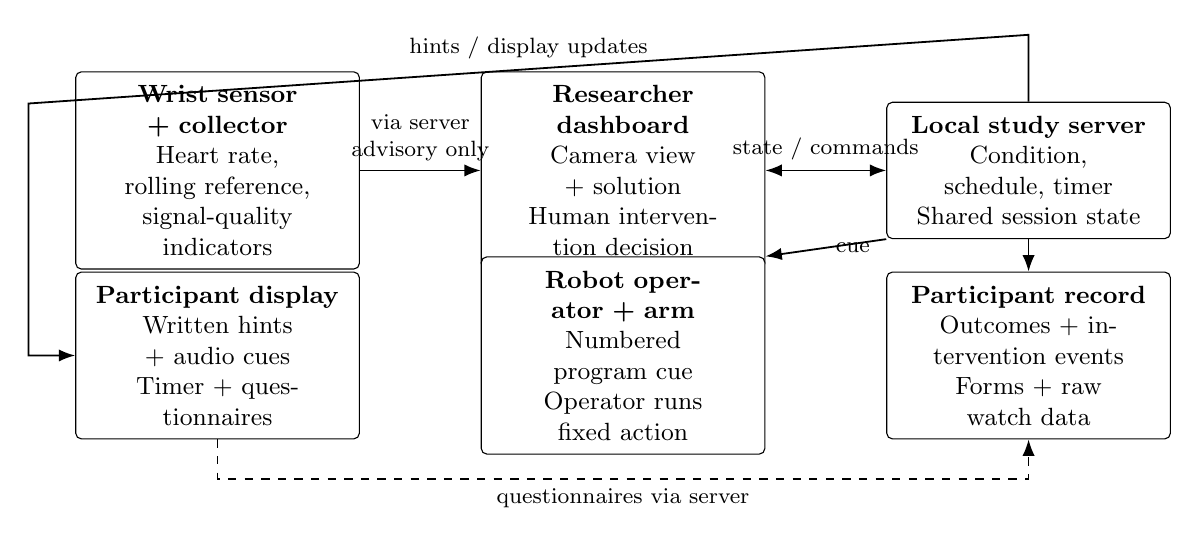
\begin{tikzpicture}[font=\small, >=Latex,
 box/.style={draw, rounded corners=2pt, align=center, fill=white,
 minimum height=1.05cm, text width=3.25cm, inner sep=5pt},
 edge/.style={->,line width=.65pt}]
\node[box] (watch) at (0,0) {\textbf{Wrist sensor + collector}\\Heart rate, rolling reference,\\signal-quality indicators};
\node[box] (wizard) at (5.15,0) {\textbf{Researcher dashboard}\\Camera view + solution\\Human intervention decision};
\node[box] (host) at (10.3,0) {\textbf{Local study server}\\Condition, schedule, timer\\Shared session state};
\node[box] (participant) at (0,-2.35) {\textbf{Participant display}\\Written hints + audio cues\\Timer + questionnaires};
\node[box] (robot) at (5.15,-2.35) {\textbf{Robot operator + arm}\\Numbered program cue\\Operator runs fixed action};
\node[box] (logs) at (10.3,-2.35) {\textbf{Participant record}\\Outcomes + intervention events\\Forms + raw watch data};
\draw[edge] (watch) -- node[above,align=center,font=\footnotesize]{via server\\advisory only} (wizard);
\draw[<->,line width=.65pt] (wizard) -- node[above,font=\footnotesize]{state / commands} (host);
\draw[edge] (host) -- (logs);
\draw[edge] (host.south west) -- node[right,font=\footnotesize]{cue} (robot.north east);
\draw[edge] (host.north) -- ++(0,.85) -- node[above,font=\footnotesize]{hints / display updates} (-2.4,.85) -- (-2.4,-2.35) -- (participant.west);
\draw[edge,dashed] (participant.south) -- ++(0,-.5) -| node[pos=.25,below,font=\footnotesize]{questionnaires via server} (logs.south);
\end{tikzpicture}
\caption{The implemented Wizard-of-Oz system. Solid arrows show assistance and state flow; the dashed route represents questionnaire capture. The server links physiological data and study events to the participant record. Human operators retain intervention selection and robot execution. The camera supports researcher observation, not automated task-progress inference.}
\label{fig:architecture}
\Description{Six boxes on a white background represent the wrist sensor and collector, researcher dashboard, local server, participant display, robot operator and arm, and participant record. Sensor cues reach the researcher through the server. The researcher issues commands, and the server distributes hints and robot-program cues and records study data.}
\end{figure*}



\subsection{Informational and physical assistance}

Informational assistance takes the form of on-screen text, accompanied by an audible notification. The configuration includes puzzle-specific hints about piece location, orientation, and adjacency. For example, a hint may identify the region occupied by a large triangle or suggest orienting the square as a diamond. The dashboard makes these hints available to the researcher, who determines which one to send.

Physical assistance is requested through a piece-specific control. Each of the seven colored pieces is mapped to a fixed robot program. The robot-operator screen displays the corresponding instruction, and the operator executes that program. Pieces not in use are returned to marked starting locations, with their centers aligned to the corresponding dots, because the robot's pickup actions depend on those locations. The robot brings a selected piece; the participant remains responsible for assembling the target configuration.

\subsection{Physiological capture and processing}

The implementation receives heart-rate measurements from a Maxim H Band over Bluetooth Low Energy. A Python collector decodes incoming measurements, retains the raw notifications, and exposes processed information to the study application. The researcher dashboard presents heart rate, available heart-rate-variability measures, and separate guidance about signal quality. A Logitech C270 camera provides a workspace view for researcher observation; this view is not an automated estimate of puzzle progress.

The live arousal cue compares recent heart rate with a preceding reference window. At the inspected version's default settings, the current value is the median of usable heart-rate samples from the most recent 15 seconds. The reference is the median from the preceding 60 seconds, excluding the current window. When that reference contains fewer than ten usable samples, a previously calibrated baseline is used if available. A rise of at least 5 beats per minute produces a possible-arousal cue, provided the current window passes the heart-rate quality check. The current window requires at least five usable samples. Values outside 30--240 beats per minute and measurements explicitly reporting poor contact are excluded; where contact information exists, the current window must also have no more than 20\% poor-contact packets.

The collector supports a 60-second baseline period and researcher-requested recalibration. Baseline completion additionally requires sufficient heart-rate samples and beat intervals. Heart-rate variability is treated separately from the live heart-rate-rise cue: the presence of an HRV value does not establish that the underlying intervals are reliable. The system's quality checks are implementation safeguards, not a validation of stress inference.

\subsection{Assistance conditions}

\textbf{No assistance.} Participants work on the tangram without task hints or robot movements. The application disables the assistance controls for this condition. The timer, task-outcome recording, and post-puzzle workload questionnaire remain part of the study procedure.

\textbf{Scheduled assistance.} The researcher receives a recurring time-based reminder and delivers assistance according to the scheduled protocol. The interface's default reminder interval is 30 seconds. The reminder does not itself send a hint or execute a robot program, so the delivered interventions depend on researcher action. We use \emph{scheduled} for this condition throughout the paper; the software labels it \texttt{constant}.

\textbf{Physiology-informed adaptive assistance.} The researcher considers heart-rate cues alongside observation of the participant's task progress when deciding whether to help. The dashboard highlights possible arousal during adaptive rounds, but neither the cue nor its absence mandates an intervention. The researcher selects and sends the hint and/or robot cue. Adaptation therefore occurs through the researcher-mediated decision process.

\section{Study Design and Measures}

\subsection{Design and participants}

The study uses a within-participant design comparing the three assistance conditions. Each participant attempts nine distinct puzzles in three consecutive sittings of three puzzles each. One condition applies throughout a sitting, and each participant experiences every condition. The study involves 24 participants (N = 24).

Recruitment uses an online form that describes the nine-puzzle activity, wrist sensing, workspace video recording, and questionnaires. It collects contact information for scheduling, age, gender, occupation or academic role, prior participation in a similar experiment, previous experience interacting with robots, availability, willingness to be recorded, and consent to participate. The form states that the recording excludes the participant's face. These questions provide participant background and recruitment information; they do not measure a preference for tangrams over alternative tasks. Immediately before the experiment, the application collects an expected-efficacy rating for robot assistance, alongside demographics, instruction acknowledgement, and consent.

The application cycles through all six permutations of condition order using the participant identifier. It also permits a manually specified order. Independently, the nine puzzles are shuffled with a participant-specific seed and divided into three consecutive sets of three. The order and seed are saved with the participant record. This procedure varies the association between puzzle identity, sitting, and assistance condition; it does not guarantee equal puzzle difficulty across conditions in the realized sample.

\subsection{Procedure}

Before the first puzzle, the participant receives the study instructions, acknowledges them, provides consent, enters demographic information, and rates their expected efficacy of robot assistance. The researcher maintains a separate profile entry that the application checks against the participant entry. The instructions explain use of all seven pieces, return of unused pieces to their marked locations, the availability of different forms of help, and the ability to pause or stop participation.

The researcher starts each puzzle round when the participant begins work. A countdown remains visible on the participant screen; the software supports audible cues at the start, midpoint, and end of the allotted time. The researcher can pause and resume the timer. Each puzzle has a five-minute time limit. At the end of a round, the researcher explicitly records whether the puzzle was solved. Participants then complete the questionnaire for that round before progressing. Breaks separate the first and second sittings and the second and third sittings. After the ninth puzzle, participants complete the overall questionnaire and may leave a written comment.

\subsection{Task performance}

The primary task records are the researcher-entered outcome and the elapsed duration of each puzzle attempt. In the ordinary round-completion path, duration is the interval between start and completion after subtracting recorded pauses. A successful attempt provides a time to completion. For an unsuccessful attempt, elapsed time represents time spent working, not a successful completion time. These quantities must remain distinct when comparing conditions.

The stored record distinguishes solved, not solved, skipped, and unrecorded outcomes. It also retains timing and intervention events. A full nine-puzzle protocol provides three attempted puzzles per condition per participant; actual denominators depend on completion of the protocol. Intervention timestamps and types permit the amount of delivered assistance to be described alongside performance, rather than assuming that nominal condition labels imply equal exposure.

\subsection{Per-puzzle experience}

After every puzzle, participants answer six adapted NASA-TLX questions covering mental demand, physical demand, temporal demand, perceived performance, effort, and frustration \cite{hart1988}. Each response is an integer from 1 to 7. Higher values indicate greater demand, effort, or frustration on the corresponding items; the performance item instead runs from failure to perfect performance. The scale direction is preserved when reporting the individual dimensions.

After puzzles in either assisted condition, four additional questions address combined helpfulness of the text and robot movements, appropriateness of intervention timing, disruption of focus, and perceived relief of frustration when stuck. Higher scores indicate more favorable experiences on all four items. In particular, the disruption question runs from highly disruptive to completely seamless. Although the software calls the last item \texttt{stressReduction}, its wording asks about frustration, so it is reported as perceived frustration relief.

These four items are absent in the no-assistance condition. Comparisons of helpfulness and timing therefore concern the two assisted conditions. The helpfulness question evaluates text hints and robot movements together; it does not identify their separate contributions.

\subsection{Overall assessment}

At the end of the study, participants rate overall helpfulness, overall efficacy, trust in useful and appropriate robot assistance, and their tendency to follow guidance even when uncertain it is correct. Responses again use seven-point scales. An optional free-text field allows participants to describe their experience in their own words. The uncertainty item is a self-report of following guidance, not a behavioral test of automation bias. Because these questions are asked once after all conditions, they characterize the overall experience rather than separate condition-specific trust scores.

\subsection{Data capture and traceability}

Each participant's record links the condition order, puzzle schedule, round outcomes and durations, assistance events, and questionnaire responses. The application continuously writes a session export, a questionnaire-only export, an event timeline, and raw watch notifications with study context. This structure permits the correspondence between a questionnaire and its preceding puzzle to be checked and supports inspection of the intervals between physiological cues and intervention commands.

Researcher overrides, including skipped questionnaires, can be recorded with reasons. Camera recording is optional and must be distinguished from the live camera view. Likewise, an application timestamp for a robot cue is a command timestamp rather than a measured onset of physical movement. Any analysis requiring actual movement onset or successful delivery needs corroboration from the relevant recording or an additional execution record.
% Results, discussion, limitations and conclusion intentionally unwritten.
\bibliographystyle{ACM-Reference-Format}
\bibliography{references}
\end{document}
